\chapter{Implementation}

\section{Design Considerations}
=== Scratch programs depend on real time
- Scratch blocks that involve timings, like "wait" or "say for secs" use real time to delay execution
$\rightarrow$ Scratch programs can not be sped up for testing
$\rightarrow$ Since Scratch 3.0 runs in a single-threaded environment (JavaScript), running multiple instances
              at once will influence the execution

=== Seeing test output, interactive tests
- Users will want to see the program's output while it is run to check if the tests run correctly
    - Difficult to determine a problem with the project from just textual test reports
$\rightarrow$ Has to be able to run in a interactive environment
    - Web GUI, which can be run by any modern browser
    - Allows users to run individual tests on the project and see the program execution

=== Batch Testing of Projects
- Some tests for Scratch projects can take a long time because projects run in real time
    - raises the need to test scratch programs in parallel
    - Scratch depends on the renderer
        - Some functionality of the Scratch virtual machine depends on the renderer
        - Headless tests are impossible without restricting the Scratch program to a subset of available blocks
$\rightarrow$ Web GUI has the option to run tests on multiple projects sequentially, but this might still take a long time depending on the project and the test suite
$\rightarrow$ Electron
    - Running tests in multiple processes could circumvent the problem
    - Electron provides a renderer that can be used to render the Scratch output to
    - Spawns multiple processes which open a window each, one project is tested in each window

=== Some tested properties will depend on time
- A tested property might depend on a previous value
    - e.g. check if a sprite is moving right
    - sprites save the values from the previous execution step
- Some tested properties should hold for a time or for the whole execution
    - Provide a way to define constraints that must always hold

\section{Implementation}
- Implemented in JavaScript as Scratch 3.0 is implemented in JavaScript

\begin{figure}
    \centering
    \tikzset{>=latex,
             label/.style={draw=none, text width=5.3cm, minimum height=0.5cm, text centered},
               box/.style={draw,      text width=2.5cm, minimum height=0.7cm, text centered, rounded corners},
                 h/.style={fill=blue!10}}

    \begin{tikzpicture}
        \node[box] at ( 0.0,  3.0) (testfw)        {Test Framework};
        \node[box]   at ( 0.0,  1.5) (testdriver)    {Test Driver};
        \node[label] at ( 0.0,  0.0) (vmwrapper)     {VM Wrapper};
        \node[box]   at (-1.4, -0.7) (sprites)       {Sprites};
        \node[box]   at (-1.4, -1.6) (inputs)        {Inputs};
        \node[box]   at ( 1.5, -0.7) (callbacks)     {Callbacks};
        \node[box]   at ( 1.5, -1.6) (constraints)   {Constraints};
        \node[box]   at (-2.0, -3.2) (scratchvm)     {Scratch VM};
        \node[box]   at ( 2.2, -3.2) (scratchrender) {Renderer};

        \begin{scope}[on background layer]
            \node[draw, h, rounded corners, fit=(vmwrapper)(sprites)(inputs)(callbacks)(constraints)] (container) {};
        \end{scope}

        \foreach \pp/\pf/\pt in {--/testfw/testdriver,
                                 --/testdriver/container,
                                 --/container/scratchvm,
                                 --/container/scratchrender,
                                 --/scratchvm/scratchrender}
        \draw[shorten >= 2pt, ->] (\pf) \pp (\pt);
    \end{tikzpicture}

    \caption{Components of Whisker}
    \label{fig:components_of_whisker}
\end{figure}

\begin{figure}
    \centering
    \tikzset{>=latex,
             box/.style={draw, text width=4.3cm, minimum height=0.7cm, text centered, rounded corners},
             num/.style={draw, circle, inner sep=0.6mm, text centered},
               h/.style={fill=blue!10}}

    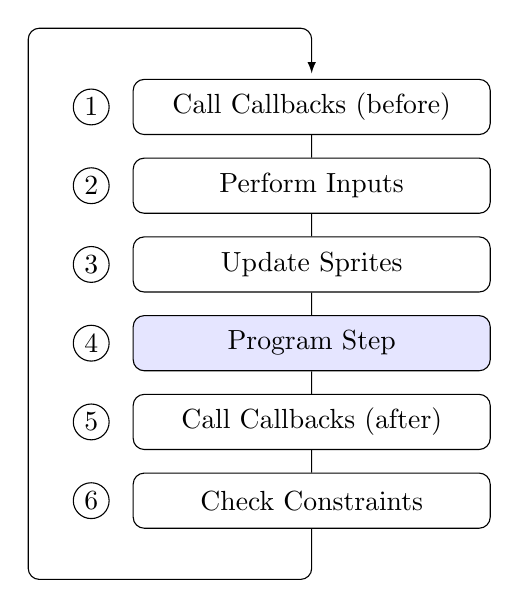
\begin{tikzpicture}
        \node[box]    at ( 0.2,  5.0) (callbacksbefore)    {Call Callbacks (before)};
        \node[box]    at ( 0.2,  4.0) (inputs)             {Perform Inputs};
        \node[box]    at ( 0.2,  3.0) (sprites)            {Update Sprites};
        \node[box, h] at ( 0.2,  2.0) (step) {Program Step};
        \node[box]    at ( 0.2,  1.0) (callbacksafter)     {Call Callbacks (after)};
        \node[box]    at ( 0.2,  0.0) (constraints)        {Check Constraints};

        \node[num] at (-2.6,  5.0) (one)   {1};
        \node[num] at (-2.6,  4.0) (two)   {2};
        \node[num] at (-2.6,  3.0) (three) {3};
        \node[num] at (-2.6,  2.0) (four)  {4};
        \node[num] at (-2.6,  1.0) (five)  {5};
        \node[num] at (-2.6,  0.0) (six)   {6};

        \draw[shorten >= 2pt, rounded corners, ->]
            (callbacksbefore)
            -- (inputs)
            -- (sprites)
            -- (step)
            -- (callbacksafter)
            -- (constraints)
            -- ( 0.2, -1.0)
            -- (-3.4, -1.0)
            -- (-3.4,  6.0)
            -- ( 0.2,  6.0)
            -- (callbacksbefore);
    \end{tikzpicture}

    \caption{Step Loop}
    \label{fig:step_loop}
\end{figure}

\section{Running Tests}
- Whisker comes with an optional testing framework
- Include a sample test report?
